\setchapterstyle{kao}
\setchapterpreamble[u]{\margintoc}
\chapter{Jointly learning model structure and compositional operations}
\labch{tree}

% \newcommand{\bcomment}[2]{{\bfseries\color{red} #1} {\bfseries\color{blue}#2}}

\cleanchapterquote{Give orange me give eat orange me eat orange give me eat orange give me you.}{Nim Chimpsky}{Male chimpanzee, 1979}

% \bcomment{}{Yep. the neural models cannot handle quantification naturally. Change the example to sentiment analysis and maybe refer to previous chapters on differences between logical representations and neural representations. Problematize : You might also state what gains you expect from structuring a neural model with a tree shape rather than using say an LSTM.}

This chapter examines the possibility of including tree-like structural bias in neural models while minimizing or eliminating direct structure supervision. 

There is this strong hypothesis in computational linguistics that language has a recursive structure \parencite{chomsky_56}. Thus, computing sentence semantic representations traditionally calls for a recursive compositional function whose structure is tree-shaped. As illustrated in \reffig{tree:tree-expl}, we can use a sentence structure as support to compute semantic representations—in this case, FOL statements, as introduced in \refsec{meaning:formal}. When using vector representations, we can also use the structure as support to encode the sentence. Following this direction, \textcite{socher_13} introduce the Stanford sentiment treebank: a corpus with fully labeled parse trees that can be used to analyze the compositional effects of sentiment in language. The dataset provides fine-grained information about lexical units carrying positive or negative sentiment. As illustrated in \reffig{tree:tree-expl}, a sentiment prediction system cannot predict the sentiment of a given sentence by simply averaging the sentiment carried by each word. We can only infer this sentiment by analyzing the sentence's structure together with individual words.

\begin{figure*}[htb!]
    \centering
    \begin{subfigure}[b]{8cm}
        \centering
        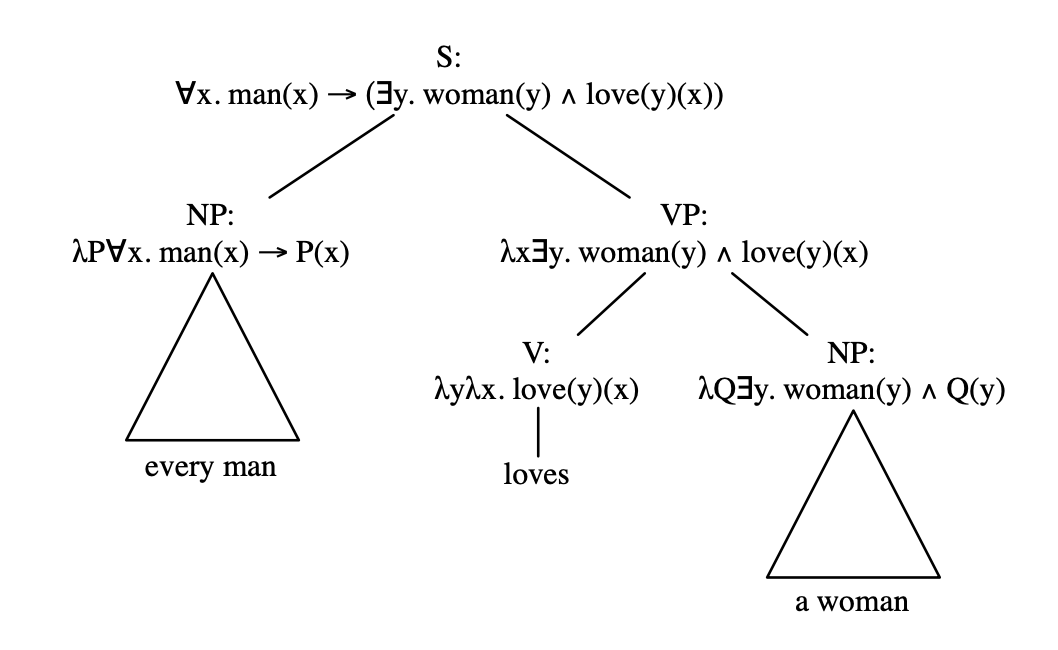
\includegraphics[width=7.5cm]{images/lambda_form.png}
    \end{subfigure}
    \hfill
    \begin{subfigure}[b]{8cm}  
        \centering 
        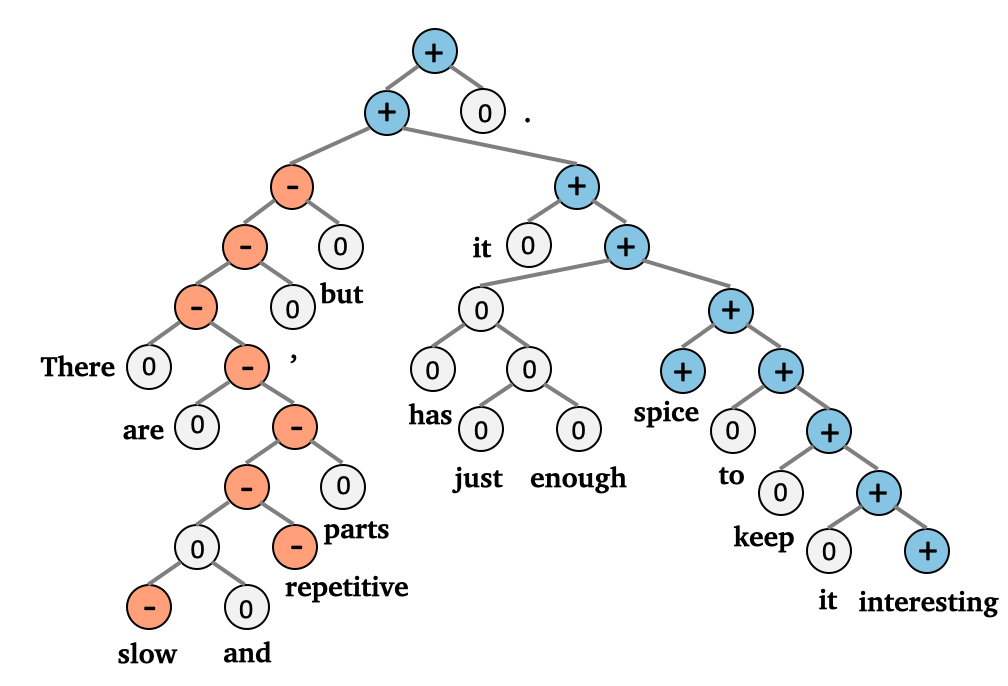
\includegraphics[width=7.5cm]{images/socher-tree-5.png}
\end{subfigure}
\caption{\labfig{tree:tree-expl}\textit{(left)} We illustrate a Montague-style \parencite{montague_1973} derivation of a semantic representation for the sentence "Every man loves a woman." We extracted the figure from \url{https://www.coli.uni-saarland.de/~koller/papers/sem-handbook.pdf}. \textit{(right)} We extracted a sentence from the Stanford sentiment treebank. The sample provides annotation for each word contribution to the final sentence sentiment. There are two parts in the sentence "There are slow and repetitive parts, but it has just enough spice to keep it interesting.", respectively negative and positive. The final sentence ends up positive. We adapted the figure from \url{http://nlp.stanford.edu:8080/sentiment/rntnDemo.html}.}
\end{figure*}

\textcite{socher_13} propose to combine the Stanford sentiment treebank with recursive neural networks. We already introduced such architectures in \refsec{architectures:tree} and successfully used them in \refch{structure-scale}. Recursive neural networks represent a phrase using word vectors and a parse tree. They compute parent vectors in a bottom-up fashion using the children as input arguments from a composition function. The composition function is shared across all node computations. \textcite{socher_13} show that, unlike bag of words, recursive networks can capture the scope of negation and sentiment change induced by contrastive conjunctions such as "but".

However, not everyone has access to resources as rich as the Stanford sentiment treebank. The corpus is only available in English and requires precise annotations from experts in linguistic. This chapter investigates the possibility of incorporating tree structural biases with minimal explicit supervision. To this end, we propose a model that jointly parses sentences into discrete trees and composes a semantic vector along with these trees.

We organize our chapter as follows: \refsec{tree:related-work} reviews related models, learning the composition function together with the sentence structure. \refsec{sec:model} introduces our model, which is based on well-known components and could therefore accommodate a variety of parsing architectures such as graph parsers or attention matrices from \textsc{Bert}. In \refsec{sec:eval}, we train and evaluate the full model with distant downstream supervision on textual entailment and semantic similarity tasks. Finally, in \refsec{sec:parser-init}, we analyze how the initial parser supervision impacts the learned structures and the performance on downstream tasks.


% Using syntax driven semantic analysis \parencite{jurafsky_2009}, we can map a sentence to a logical form that reflects its meaning—following the definition from \refsec{meaning:formal}. In this perspective, \bcomment{nonsense}{} we compute the sentence meaning using the compositionality principle. In its essence, the principle states that we can derive the meaning of a sentence by composing the meaning of its parts. \bcomment{That's an operational statement}{} We first infer the sentence structure\sidenote{The structure may consist in various trees such as constituency, dependency or binary parses.}. We then recursively compute the semantic representation along the structure, by \bcomment{rephrase the sentence}{} augmenting and combining each node with semantic attachments. These attachments follow explicit combination rules.





% We propose a framework relying explicitly on syntactic trees rather than analyzing the patterns learned by statistical models. 

% To compute semantic representations, tree structured models rely on an explicit and discrete structure. It favors the integration of linguistic information and inductive biases. Moreover, it favors the analysis of the composition since it explicitly relies on syntactic trees. Yet, such models require \bcomment{raw text and linguistic structure}{not only raw text but also linguistic structure} in the form of parse trees to calculate the semantic representation. This prerequisite limits their use in practice \bcomment{}{because it requires annotations in the supervised case}. By using tree structure neural models without the need for labeled parses, we hope to overcome this limitation.

% We evaluate our model on textual entailment and semantic similarity tasks and outperform sequential models and tree-structured models relying on external parsers. Moreover, when initialized on human-annotated structures, our model improves inference close to \textsc{Bert} base performances on the semantic similarity task. 

% We then conduct an ablation study to quantify the impact of the parser initialization on the resulting structures and downstream performances. We corroborate that the sole use of downstream supervision is insufficient to produce parses that are easy to interpret. To encourage convergence towards readable linguistic structures, we examine a number of initialization setups. We observe that our structures often converge toward trivial branching patterns, which have few in common with gold linguistic parses. However, with respect to the downstream performances, linguistic insights appear as a relevant initialization.

% \section{Principle of compositionality for building semantic representations}

% \begin{figure}[htb!]
% 	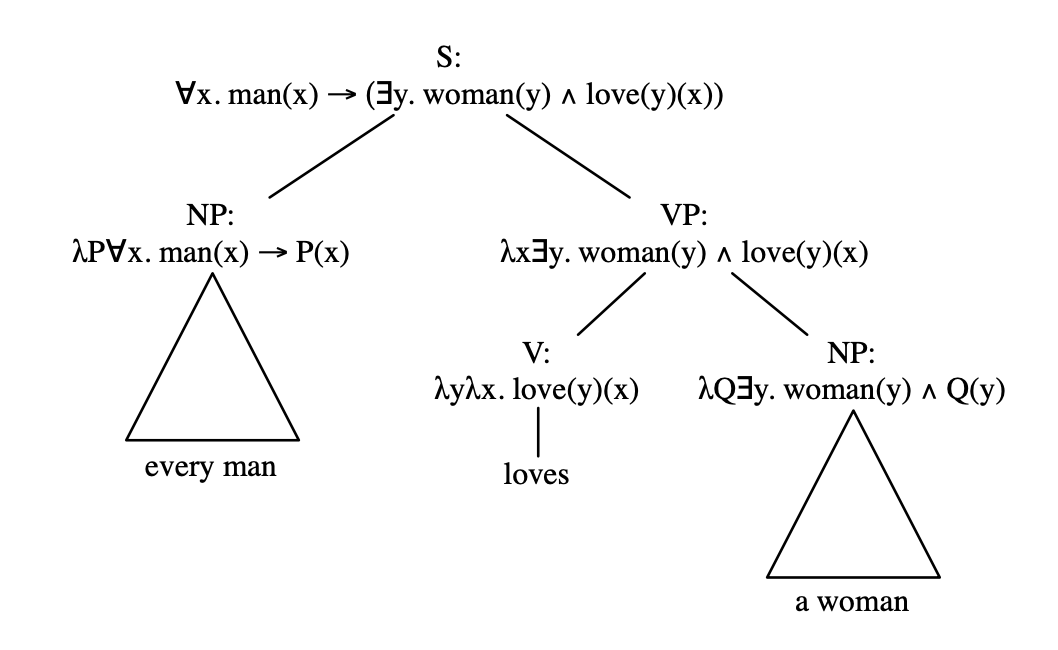
\includegraphics[width=10cm]{images/lambda_form.png}
% 	\caption[Lambda form]{A Montague-style \parencite{montague_1973} derivation of a semantic representation for the sentence “Every man loves a woman.” Credits: by Alexander Koller and Manfred Pinkal \url{https://www.coli.uni-saarland.de/~koller/papers/sem-handbook.pdf}}
% 	\labfig{lambda-form}
% \end{figure}

% There is this strong \bcomment{intuition}{hypothesis} \bcomment{in natural language processing}{computational linguistics} that language has a recursive structure \parencite{chomsky_56, shen_19}. As illustrated in \reffig{lambda-form} computing sentence semantic representations traditionally calls for a recursive compositional function whose structure is tree-shaped. Using syntax driven semantic analysis \parencite{jurafsky_2009}, we can map a sentence to a logical form that reflects its meaning—following the definition from \refsec{meaning:formal}. In this perspective, \bcomment{nonsense}{} we compute the sentence meaning using the compositionality principle. In its essence, the principle states that we can derive the meaning of a sentence by composing the meaning of its parts.
% \bcomment{That's an operational statement}{} We first infer the sentence structure\sidenote{The structure may consist in various trees such as constituency, dependency or binary parses.}. We then recursively compute the semantic representation along the structure, by \bcomment{rephrase the sentence}{} augmenting and combining each node with semantic attachments. These attachments follow explicit combination rules.

% \begin{figure}[htb!]
% 	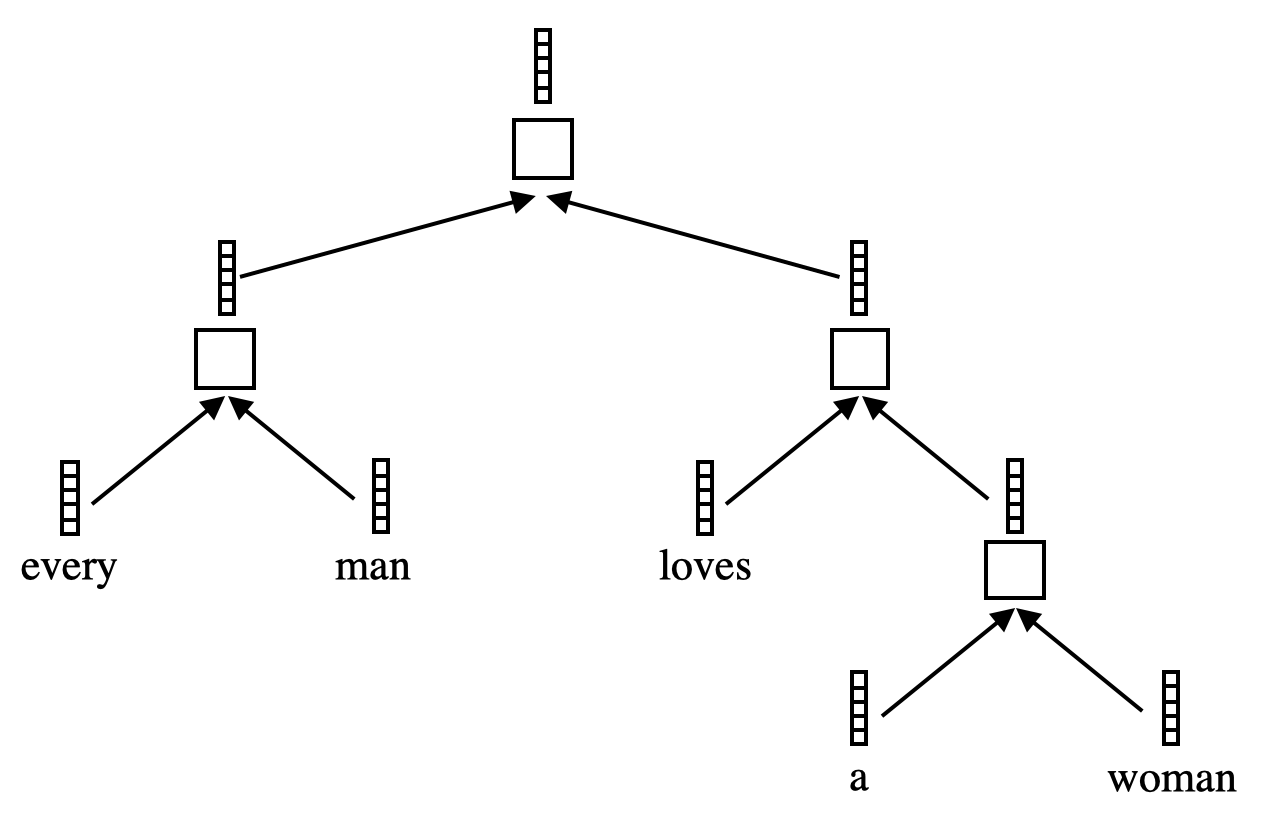
\includegraphics[width=10cm]{images/tree_rnn.png}
% 	\caption[Tree LSTM]{Semantic encoding of a sentence using a tree-structured neural model.}
% 	\labfig{tree-rnn}
% \end{figure}

% As detailed in \refsec{training:architectures}, computing sentence semantic representations traditionally calls for a recursive compositional function whose structure is tree-shaped. 
% \bcomment{}{Yep. the neural models cannot handle quantification naturally. Change the example to sentiment analysis and maybe refer to previous chapters on differences between logical representations and neural representations. Problematize : You might also state what gains you expect from structuring a neural model with a tree shape rather than using say an LSTM.} Neural models can emulate this composition procedure using tree-structured networks. As for the logical form, such models proceed in two stages: first we infer the syntactic structure of the sentence, then we recursively compose the semantic representation along the structure. We illustrate the composition procedure in \reffig{tree-rnn}. Here, the semantic representations consist of vectors composed with linear algebra operations—as detailed in \refsec{meaning:distributional}. The parameters of the semantic algebraic operators are \textit{learned} by optimizing a loss function given a dataset. Regarding the sentence structure, we usually infer it using a dedicated parser, learned on labeled data.

% and enable better generalization and abstraction properties.

%%%%%%%%%%%%%%%%%%%%%%%%%%%%%%%%%%%%%%%%%%%%%%%%%%%%%%%%%%%%%%%%%%%%%%%%%%%%%%%%
\section{Latent tree learning}
\labsec{tree:related-work}
%%%%%%%%%%%%%%%%%%%%%%%%%%%%%%%%%%%%%%%%%%%%%%%%%%%%%%%%%%%%%%%%%%%%%%%%%%%%%%%%

Tree-structured models rely on an explicit and discrete structure to compute semantic representations. It favors the integration of linguistic information and inductive biases. Moreover, it favors compositional analysis since it explicitly relies on syntactic trees. However, such models require not only raw text but also linguistic structure in the form of parse trees to calculate the semantic representations. This prerequisite limits their use in practice because it requires annotations in the supervised case. 
% By using tree structure neural models without the need for labeled parses, we hope to overcome this limitation.

% \bcomment{not really true}{in the supervised setting} Tree-based models need carefully hand-annotated data to be trained. 
One method of overcoming this limitation is to induce trees from raw text and computes semantic representations along with the inferred structure. Such a method preserves explicit recursive computations and produces intelligible tree structures. Known as \textit{latent tree learning}, these methods generally consist of two components: a parser and a composition function that uses the parses. The parser and composition function are learned jointly and are specific to a given task or domain. 
% The learning method is called \textit{latent tree learning}, and it \bcomment{usually}{that's not usual} consists of two components: a parser and a \textsc{TreeLSTM} that uses those parses. 

% All models differ from the syntactic formalism used and the training method.

The first set of latent tree models introduces an intermediate objective to train the parser component. \textcite{socher_11c} parse the sentence by selecting and merging adjacent nodes. The parser model is trained using an auxiliary reconstruction task. The Shift reduce Parser-Interpreter Neural Network (SPINN) model from \textcite{bowman_16} obtains the structure using a shift-reduce parser. The parser component also uses an intermediate objective that compares parses with gold-standard trees.

% defines a relaxation of a CYK-like chart parser 
\textcite{maillard_19} explicitly compute a whole forest of
%$\mathcal{O}(N^2)$ \bcomment{incorrect combinatorics}{}
potential binary parse trees for a sentence of $N$ words. 
%\sidenote{The number of possible binary trees with $n-1$ leafs is given by the nth Catalan number, $C_n = \frac{(2n)!}{(n+1)!n!} \sim \frac{4^n}{\sqrt{\pi}n^{\frac{3}{2}}$ \parencite{vardi1991computational}.}
All possible partial trees of a sentence are stored in a chart data structure inspired by the CYK parser. The final tree is constructed as a soft combination of the constituents available in each chart cell, thus approximating discrete candidate selection and making the model entirely trainable using backpropagation. However, the linear increase in candidates with depth makes this algorithm memory intensive.


% \textcite{maillard_19} introduce a model entirely trainable using backpropagation. However, the model does not rely on a soft structure and does not maintain the discreteness of the tree composition process\bcomment{a bit elliptic. what do they do really ?}{more details would be welcome}. It is, therefore, memory intensive as it explicitly computes a whole forest of 
% % $\smallO{N^2}$ 
% potential trees. 
% %for $N$ words

% \citet{yogatama_17} is the first model to jointly train its parsing and sentence embedding components. They base their model on shiftreduce parsing. Their parser is not differentiable, so they rely on reinforcement learning for training.

% \citet{yogatama_17} adapt the Spinn model with the REINFORCE algorithm. \citet{yogatama_17} introduce reinforcement learning to achieve the desired effect of discretization. However, slow convergence due to the reinforcement learning setting is one of its draw- backs, according to the authors.

% Our main idea is to use reinforcement learning (policy gradient methods) to discover the best tree structures for the task that we are interested in. We do not place any kind of restrictions when learning these structures other than that they have to be valid binary parse trees, so it may result in tree structures that match human linguistic intuition, heavily right or left branching, or other solutions if they improve performance on the downstream task. We parameterize each action a ∈ {SHIFT, REDUCE} by a policy network
% guided composition orders of Tree LSTM models are given directly as input

\textcite{yogatama_17} adapt the training of the \textsc{SPINN} model to make it fully differentiable. As such, the model does not require any structure supervision during training. Instead of providing the model with the parse of the input, the procedure uses reinforcement learning (policy gradient methods) to discover the best tree structures for the task. However, the reinforcement learning strategy is notoriously slow and limits the convergence speed.

% \textcite{yogatama_17} adapt \textsc{SPINN} and jointly train its parsing and sentence embedding components. The model produces a discrete structure, but the resulting architecture is not fully differentiable and must thus be trained using a reinforcement learning proxy objective, limiting the convergence speed. 

% \citet{choi_18} use an approach similar to easy-first parsing. The parsing decisions are discrete, but the authors use the Straight-Through Gumbel-Softmax estimator to obtain an approximate gradient and are thus able to train with backpropagation.

% \citet{choi_18} present a model (ST-Gumbel) that uses a similar data structure and gating strategy to \citet{maillard_19}, but which uses the Straight-Through Gumbel-Softmax estimator. This allows them to use a hard categorical gating function, so that their output sentence vector is computed according to a single tree, rather than a gated combination of partial trees as in \citet{maillard_19}.

% \textcolor{blue}{ \citet{choi_18} compute a single tree instead of combinations from partial trees by using the Straight-Through Gumbel-Softmax estimator. The input is greedily and sequentially parsed.}
% . However, \citet{choi_18} model iterates through $N - 1$ steps to build a tree over $N$ words, }

\textcite{choi_18} propose a method that is both fully differentiable and maintains the discreteness of the parsing process. Contrary to \textcite{yogatama_17}, it does not require the reinforcement learning artifice for training; contrary to \textcite{maillard_19}, it computes a single discrete tree instead of combinations from partial trees. The methods proceed in $N - 1$ iterations to build a tree over $N$ words. Using the Gumbel-Softmax estimator, two nodes are selected from the available candidates at each iteration. During the forward pass, the estimator is used as a discrete argmax function to select nodes to merge. During the backward pass, The estimator relaxes the discrete sampling operation so that it can be trained with backpropagation.

% compute a single tree instead of combinations from partial trees by using the Gumbel-Softmax estimator. The input is greedily and sequentially parsed.
% \bcomment{overall at the end of this section, I miss some more details on what these guys really do. It requires to read the papers to get an idea. Lacks of self containment}{}


% a reconstruction error in \citet{socher_11c} and a comparison with gold-standard trees in \citet{bowman_16}.}

%A \treelstm{} is then applied on the parse to embed the sentence. But both models train the parser with an auxiliary task.
%: a reconstruction error and a comparison with gold-standard trees.

% \citet{bowman_16} introduce the Shift-reduce Parser-Interpreter Neural Network (SPINN). However as in \cite{socher_11c} the model train the parsing module with an auxiliary loss to match gold-standard trees. 

%%%%%%%%%%%%%%%%%%%%%%%%%%%%%%%%%%%%%%%%%%%%%%%%%%%%%%%%%%%%%%%%%%%%%%%%%%%%%%%%%%%%%%%%
% 2. Yogatama
%%%%%%%%%%%%%%%%%%%%%%%%%%%%%%%%%%%%%%%%%%%%%%%%%%%%%%%%%%%%%%%%%%%%%%%%%%%%%%%%%%%%%%%%

% \citet{yogatama_17} is the first model to jointly train its parsing and sentence embedding components. They base their model on shiftreduce parsing. Their parser is not differentiable, so they rely on reinforcement learning for training.

% \citet{yogatama_17} adapt the Spinn modelwith the REINFORCE algorithm. \citet{yogatama_17} introduce reinforcement learning to achieve the desired effect of discretization. However, slow convergence due to the reinforcement learning setting is one of its draw- backs, according to the authors.

%%%%%%%%%%%%%%%%%%%%%%%%%%%%%%%%%%%%%%%%%%%%%%%%%%%%%%%%%%%%%%%%%%%%%%%%%%%%%%%%%%%%%%%%
% 4. Maillard
%%%%%%%%%%%%%%%%%%%%%%%%%%%%%%%%%%%%%%%%%%%%%%%%%%%%%%%%%%%%%%%%%%%%%%%%%%%%%%%%%%%%%%%%
% \citet{maillard_19} propose an alternative approach, inspired by CKY parsing. The algorithm is made differentiable by using a soft-gating approach, which approximates discrete candidate selection by a probabilistic mixture of the constituents available in a given cell of the chart. This makes it possible to train with backpropagation.

% \citet{maillard_19} present a model, entirely trainable using  backpropagation — which explicitly computes O(N2) possible tree nodes for N words, and uses a soft gating strategy to approximately select valid combinations of these nodes that form a tree. Though their model reduces the ambiguity by explicitly representing a node as a weighted sum of all candidate compositions, it is memory intensive since the number of candidates linearly increases by depth.
% \textcolor{blue}{}

%%%%%%%%%%%%%%%%%%%%%%%%%%%%%%%%%%%%%%%%%%%%%%%%%%%%%%%%%%%%%%%%%%%%%%%%%%%%%%%%%%%%%%%%
% 5. Choi
%%%%%%%%%%%%%%%%%%%%%%%%%%%%%%%%%%%%%%%%%%%%%%%%%%%%%%%%%%%%%%%%%%%%%%%%%%%%%%%%%%%%%%%%

% \citet{choi_18} use an approach similar to easy-first parsing. The parsing decisions are discrete, but the authors use the Straight-Through Gumbel-Softmax estimator to obtain an approximate gradient and are thus able to train with backpropagation.

% \citet{choi_18} present a model (ST-Gumbel) that uses a similar data structure and gating strategy to \citet{maillard_19}, but which uses the Straight-Through Gumbel-Softmax estimator. This allows them to use a hard categorical gating function, so that their output sentence vector is computed according to a single tree, rather than a gated combination of partial trees as in \citet{maillard_19}.

% \textcolor{blue}{ \citet{choi_18} compute a single tree instead of combinations from partial trees by using the Straight-Through Gumbel-Softmax estimator. The input is greedily and sequentially parsed.}
% . However, \citet{choi_18} model iterates through $N - 1$ steps to build a tree over $N$ words, }

%%%%%%%%%%%%%%%%%%%%%%%%%%%%%%%%%%%%%%%%%%%%%%%%%%%%%%%%%%%%%%%%%%%%%%%%%%%%%%%%%%%%%%%%
%. 6. Williams
%%%%%%%%%%%%%%%%%%%%%%%%%%%%%%%%%%%%%%%%%%%%%%%%%%%%%%%%%%%%%%%%%%%%%%%%%%%%%%%%%%%%%%%%
% \citet{williams_18} investigate the trees produced by \citet{yogatama_17} and \citet{choi_18} when trained on two natural language inference corpora. They find that the former model induces almost entirely leftbranching trees, while the latter performs well but has inconsistent trees across re-runs with different parameter initializations.

% However, \citet{williams_18} empirically show that, Gumbel softmax produces unstable latent trees with the same hyper-parameters but different initializations, while reinforcement learning even tends to generate left-branching trees. Neither gives meaningful latent trees in syntax, but each method still obtains considerable improvements in performance. This indicates that syntax may not be the main contributor to the performance gains.
% We obtain a score close to the {\sc Spinn} model but without an explicit parsing objective. Rather we pre-trained the parsing model on the Penn Tree Bank and fine-tuned it on the SNLI task.


% We organized our paper as follows: after presenting the related in work in Section~\ref{sec:related-work}, we present our model in Section~\ref{sec:model}. 
% We then study the relevance of this framework for semantic inference and analyze the properties of such tree-structured models for downstream tasks. 
% In Section~\ref{sec:eval}, we evaluate our model on textual entailment and semantic similarity tasks. Regarding the textual similarity task, we show that our setup is competitive with \bert base, although the latest is trained on datasets many orders of magnitude larger. We then conduct an ablation study and analyze the impact of the parser initialization. In Section~\ref{sec:parses-impact}, we compare the learned structures across initializations and with interpretable annotations. In Section~\ref{sec:dowstream-impact} we study how latent structures impact performances on downstream tasks.
% with a significantly smaller training set.

% I focus on tree-structured neural networks, which naturally encode the structure of language. For each sentence, the network computes text units following a syntactic tree, starting from the leaf nodes, up to the root. However, such models suffer from practical constraints that limit their application. In particular, tree-based models not only require raw text as input but also the sentence structure in the form of a parse tree. Such structure may be tedious to obtain as it requires manual annotations and external parsers. To overcome such limitations, I formulated a novel tree-based model that learns its composition function together with its structure \parencite{simoulin_2020}. The model includes two modules, a biaffine graph parser, and a Tree-LSTM. The parsing and the composition functions are explicitly connected and, therefore, learned jointly. The method differs from previous work as the representation is not computed from the whole forest of potential trees. Moreover, training the full model directly does not require supervision from a parsing objective. The model outperforms tree-based models relying on external parsers on downstream tasks. In some configurations, it is even competitive with BERT-base model.

\section{Unified parsing and compositional model}
\labsec{sec:model}

% However, architectures often have practical limitations, requiring either complex learning paradigm such as reinforcement learning \parencite{yogatama_17} or intensive computations \parencite{maillard_19}.
The earlier architectures listed above have practical limitations, requiring either a complex learning paradigm such as reinforcement learning, intensive computations, or requiring an external parser module. The method proposed in \textcite{choi_18} overcomes these limits. However, \textcite{williams_18} investigate the latent trees produced by \textcite{yogatama_17} and \textcite{choi_18} and show neither method produces meaningful syntactic representations. The Gumbel-Softmax estimator outputs inconsistent trees across initializations while reinforcement learning outputs trivial left-branching trees. Moreover, \textcite{choi_18} produce trees by selecting and merging adjacent nodes. Therefore, it cannot directly use architectures designed for standard parsing formalisms such as dependency parsing algorithms.

% To limit the need for an external parser, w
In this section, we propose an original latent tree learning method. Besides addressing all the limitations listed above, our method relies on existing and well-known components. It is not limited to a particular parser architecture as long as it is differentiable. Ultimately, our method offers the following benefits:
\begin{itemize}
    \item infers an explicit tree structure and trains recursively a sentence embedding model within a unified architecture;
    \item provides end-to-end training by back-propagating the downstream task loss through the entire architecture;
    \item produces a discrete tree;
    \item accommodates any any graph-based dependency parser architecture.
\end{itemize}


% The \textsc{TreeLSTM} recursive composition function crucially uses a weighted sum of the child representations whose weights are provided by the parser edges, hence linking the parser outputs to the \textsc{TreeLSTM} recursion.
% \footnote{The model is illustrated in Appendix~\ref{sec:figure}.}.

% Our model jointly performs sentence parsing and the prediction of a sentence embedding. The sentence embedding is predicted by a weighted \textsc{TreeLSTM} whose tree structure is provided by a dependency parser.

% We use a standard dependency parsing structure, obtained using a graph-based biaffine dependency parser \parencite{dozat_17}. However, our model is not limited to a particular parser architecture as long as it is differentiable. This flexibility gives us the freedom to explore the impact of the parser choice. 

%\bcomment{}{State more clearly that you designed a joint model by contrasting with others} 
Our model jointly performs sentence parsing and the prediction of a sentence embedding. The sentence embedding is predicted by a \textsc{TreeLSTM} whose tree structure is provided by a dependency parser.

% \bcomment{apparent contradiction, you said earlier that using an external parser is a weakness}{}
\paragraph{Parsing model} We use a standard dependency parsing structure, obtained using a graph-based biaffine dependency parser \parencite{dozat_17}. Given an input sequence of $n$ words, the parser computes a weighted matrix of size $n \times n$ for which each coordinate $(i, j)$ is interpreted as a score for the $i$th word to be the head of the $j$th word. Given the un-normalized score matrix, the predicted tree is extracted using the MST algorithm. However, our model is agnostic to any graph-based parser architecture. This flexibility gives us the freedom to explore the impact of the parser choice (\refsec{sec:parser-init}).

The procedure is formalized in two steps. First, in Eq. \ref{eq:biaffine-1} to \ref{eq:biaffine-3},
it computes a weight matrix that is interpreted as weighted directed graph whose nodes are the sentence tokens:
%\par\noindent{\small
\begin{align}
   \text{Biaff}(x_1,x_2) &=  x_1^T U x_2 + W^{(b)}(x_1 \oplus x_2)+b^{(b)} \\
    a_k^{(dep)} &= W^{(dep)}h_k + b^{(dep)} \label{eq:biaffine-1} \\
    a_j^{(head)} &= W^{(head)}h_j + b^{(head)} \label{eq:biaffine-2}\\
    s^{(arc)}_{kj} &= \text{Biaff}(a_k,a_j) \label{eq:biaffine-3}
\end{align}%}
The second step performs parsing by computing a maximum spanning tree from the graph. As in \textcite{dozat_17}, we use the Max Spanning Tree (MST) algorithm \parencite{chu1965shortest, edmonds_67} 
%\bcomment{cite Edmonds as it is a non standard -directed- MST algorithm}{} 
to ensure the well-formedness of the tree: 
\begin{align}
 \alpha_{kj} &= \mathbb{1}_{mst(s^{(arc)}_{kj})} s^{(arc)}_{kj} \label{eq:biaffine-alpha}
\end{align}
Where $\alpha_{kj}$ is the probability of the edge linking node $j$ to node $k$. For a given node $k$, there is at most one non-zero edge leading to its governor $j$.
% weighted edge

\paragraph{Composition function}  Given a predicted tree structure, we recursively encode the sentence using a variant of the Child Sum Tree model from \textcite{tai_15} detailed below:
% \par\noindent{\small

\begin{align}
\tilde{h}_j &= \sum_{k \in C(j)} \alpha_{kj} h_k, \label{eq:treelstm-weighted} \\
i_j &=\sigma \left( W^{(i)} x_j + U^{(i)} \tilde{h}_j + b^{(i)} \right), \\
o_j &=\sigma \left( W^{(o)} x_j + U^{(o)} \tilde{h}_j + b^{(o)} \right), \\
u_j &=\tanh \left( W^{(u)} x_j + U^{(u)} \tilde{h}_j + b^{(u)} \right), \\
f_{jk} &= \sigma\left( W^{(f)} x_j + U^{(f)} h_k + b^{(f)} \right), \label{eq:treelstm-f}\\
c_j &= i_j \odot u_j + \sum_{k\in C(j)} f_{jk} \odot c_{k}, \\
h_j &= o_j \odot \tanh(c_j), \label{eq:treelstm-last}
\end{align}


% \begin{align}
% \tilde{h}_j &= \sum_{k \in C(j)} \alpha_{kj} h_k, \label{eq:treelstm-weighted} \\
% %\tilde{h}_j &= \sum_{k \in C(j)} h_k, \label{eq:treelstm-first} \\
% i_j, o_j, u_j &=\sigma \Big( W^{(i, o, u)} x_j + U^{(i, o, u)} \tilde{h}_j + b^{(i, o, u)} \Big), \\
% % o_j &= \sigma \left( W^{(o)} x_j + U^{(o)} \tilde{h}_j  + b^{(o)} \right), \\
% % u_j &= \tanh\left( W^{(u)} x_j + U^{(u)} \tilde{h}_j  + b^{(u)} \right), \\
% f_{jk} &= \sigma\left( W^{(f)} x_j + U^{(f)} h_k + b^{(f)} \right), \label{eq:treelstm-f}\\
% c_j &= i_j \odot u_j + \sum_{k\in C(j)} f_{jk} \odot c_{k}, \\
% h_j &= o_j \odot \tanh(c_j), \label{eq:treelstm-last}
% \end{align}
%}
Where in Eq.~\ref{eq:treelstm-weighted}, $C(j)$ denotes the set of children of node $j$.
% and $k \in C(j)$. 

% The \textsc{TreeLSTM} recursive composition function crucially uses a weighted sum of the child representations whose weights are provided by the parser edges, hence linking the parser outputs to the \textsc{TreeLSTM} recursion.

%\paragraph{Discussion}
We use the embedding computed by the weighted \textsc{TreeLSTM} at the root of the tree as the sentence embedding.
% The core model outputs a sentence embedding computed by a weighted \treelstm{}.  
% a compositionnaly weighted tree-{\sc lstm}
The tree shape and the edge weights are given by the best prediction of a graph parser. The equations from the \textsc{TreeLSTM} are the same than the one presented in \refsec{architectures:tree}, except for Eq.~\ref{eq:treelstm-weighted}. \textbf{Crucially, in our case, Eq.~\ref{eq:treelstm-weighted} is a \underline{weighted} sum rather than a standard sum and the weights are those $\alpha_{kj}$ provided by the parser.} The parsing model is linked to the \textsc{TreeLSTM} by the weights $\alpha_{kj}$. This architecture allows us to update jointly the parser and the \textsc{TreeLSTM} weights using only the downstream task loss. The supervision comes only from the objective of the downstream task, and no intermediate structure target is required.
% It does not require training the parser component using an auxiliary task;
%our model supervision only appears in the semantic objective and no intermediate structure target is required. 
% the architecture allows us to update the parser and \treelstm{} weights using solely the loss provided by the downstream task. 

% It therefore differs from models like {\sc Spinn} \cite{bowman_16}, which includes direct supervision from a parsing objective.

% The method described here differs from previous work as the representation is not computed from the whole forest of potential trees \citep{yogatama_17, maillard_19, williams_18, shen_18, liu_18} but instead on the single best tree while being completely differential. Thus, it can be trained using back-propagation on a supervised task for which we want to provide relevant sentence embeddings. The architecture is, in principle, generic and adaptable to any other downstream task. 

Our model, illustrated in \reffig{biaffine-tree-lstm}, is fully differentiable and preserves the discreteness of the tree composition process. It relies on a dependency parsing formalism and could accommodate any graph-based dependency parser.
%\bcomment{again it is too strong}{it requires that the parsing algorithm encode edges explicitly}
Intuitively, the model induces a direct link between the inference of the syntactic structure and the composition of the semantic representation. If a connection between two nodes $i$ and $j$ is irrelevant from a semantic standpoint, then its contribution $\alpha_{kj}$ into the construction of the hidden state $\tilde{h}_j$ (Eq.~\ref{eq:treelstm-weighted}) is likely to be marginal. When training the model, if such connection becomes too tenuous, it becomes unlikely to be selected when selecting the maximum spanning tree from the graph in equation \ref{eq:biaffine-alpha}.
% \bcomment{problems with refs to equations}{}


\begin{figure}[!ht]
	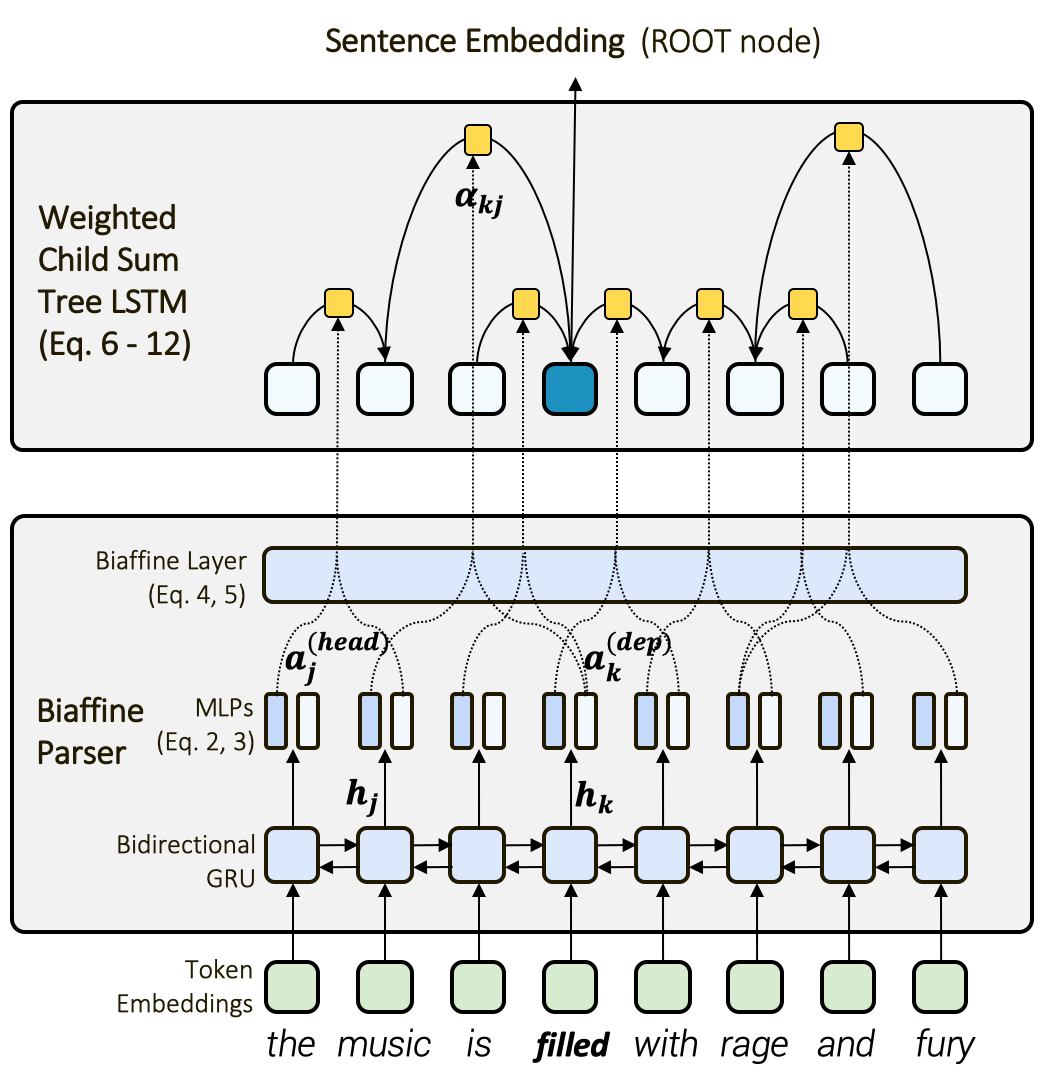
\includegraphics[width=7cm]{images/biaffine-12.png}
	\caption[Biaffine tree lstm]{We illustrate the architecture detailed in Eq. \ref{eq:biaffine-1} to \ref{eq:treelstm-last}. The Biaffine parser provides the sentence structure from which the \textsc{TreeLSTM} computes sentence embeddings. The full pipeline is differentiable as the \textsc{TreeLSTM} weights are given by the parser.}
	\labfig{biaffine-tree-lstm}
\end{figure}

%%%%%%%%%%%%%%%%%%%%%%%%%%%%%%%%%%%%%%%%%%%%%%%%%%%%%%%%%%%%%%%%%%%%%%%%%%%%%%%%
\section{Evaluation on downstream tasks}
\labsec{sec:eval}
%%%%%%%%%%%%%%%%%%%%%%%%%%%%%%%%%%%%%%%%%%%%%%%%%%%%%%%%%%%%%%%%%%%%%%%%%%%%%%%%

Our architecture primarily aims to produce relevant embeddings for downstream tasks. To this end, we compare our setup with other models from the literature on various tasks. For this comparison, we first pre-train the parsing submodel on human-annotated sentences from the Penn Tree Bank (PTB) \parencite{marcus_94} converted to Stanford dependencies. We then fine-tune the parser's parameters on the task while training the full model.\sidenote{In this configuration, we observe pre-training the parser may cause weights $\alpha$ to become too large in Eq. \ref{eq:biaffine-alpha}. This leads to poor downstream performances. We correct this with a multiplicative parameter $\tau$ whose value is estimated during training. It means we replace Eq. \ref{eq:biaffine-alpha} with: $\alpha_{kj} = \tau \cdot \mathbb{1}_{mst(s^{(arc)}_{kj})} s^{(arc)}_{kj}$ for the computation of tree weights.}


\subsection{Semantic textual similarity (STS)}
\labsec{sts}

We first evaluate our model on the SICK-R downstream task \parencite{marelli_14}, which is dedicated to assessing models' compositional properties. 
%The task intends to discriminate models that rely on shallow lexical pattern matching from those that take advantage of the sentence's underlying structure. 
The dataset comprises 9,927 sentence pairs, distributed in a \numprint{4500}/500/\numprint{4927} train/dev/test split, annotated for semantic similarity on a 1 to 5 real range. A score of 5 means that the two sentences are completely equivalent and 1 that the two sentences are completely dissimilar. In between, their degree of equivalence differs given the proportion of shared topics and information between the two sentences. The dataset includes specific examples of variations on passive and active forms, quantifier and modifier switches, or negations. We extensively present the construction of the dataset in \ref{sec:linguistic-breakdown} and give some illustration examples of the task in \reftab{senteval:examples:sick}.
%This is a SentEval task \cite{conneau_18} specifically
%\bcomment{to get a more self contained doc you might present the task with slightly more details, provide examples etc.}{}

\begin{table*}[!htb]
\footnotesize
\centering {
\begin{tabularx}{16cm}{@{}X X c@{}}
\toprule
\textbf{Sentence A} & \textbf{Sentence B} & \textbf{Target} \\
\midrule\midrule
``A man is singing a song and playing the guitar'' & ``A man is opening a package that contains headphones'' & 1.6\\[0.4cm]
``Two dogs are playing by a tree'' & ``Two dogs are playing by a plant'' & 4.6\\[0.2cm]
``A woman is riding a horse'' & ``A man is opening a small package that contains headphones'' & 1.0\\[0.4cm]
``A potato is being sliced by a woman'' & ``A woman is slicing a carrot'' & 3.0\\[0.2cm]
``A man is screaming'' & ``A man is scared'' & 3.6\\[0.2cm]
``Men are sawing logs'' & ``Men are cutting wood'' & 4.5\\[0.2cm]
\bottomrule
\end{tabularx}}
\caption{\labtab{senteval:examples:sick} SICK-R is a Semantic Textual Similarity (STS) task for which labels are scores between 1 and 5. A score of 5 means that the two sentences are completely equivalent and 1 that the two sentences are completely dissimilar. In between, their degree of equivalence differs given the proportion of shared topics and information between the two sentences.}
\end{table*}

\paragraph{Training configuration}

% \bcomment{with more details on the task, the following parag would be easier to understand}{}
We use a similar training procedure
%\footnote{Hyperparameters such as hidden size, optimization procedure such or learning rate are fixed as proposed in \citet{tai_15} and are detailed in Appendix.} 
as in \textcite{tai_15}. We transform the target $y$ from the SICK-R task into the distribution $p$ defined by:

\begin{equation*}
p_{i} = \left\{
\begin{array}{ll}
y - \lfloor{y}\rfloor, & i = \lfloor{y}\rfloor + 1 \\
\lfloor{y}\rfloor - y + 1, & i = \lfloor{y}\rfloor \\
0 & \text{otherwise}
\end{array} \right.
\end{equation*}
We use a dedicated architecture to predict the similarity distribution from a pair of sentences. The similarity module takes as input a pair of sentence vectors $h_{L} $ and $h_{L}$ and computes their component\-wise product $h_{L} \odot h_{R}$ and their absolute difference $|h_{L} - h_{R}|$. Given these features, we compute the probability distribution  $\hat{p}_{\theta}$ using a two-layer perceptron network (MLP):
\begin{align}
\begin{split}
&h_{\times}=h_L\odot h_R, ~~~~~h_{+} = |h_L - h_R |, \\
&h_s = \sigma (W^{(\times)}h_{\times} + W^{(+)}h_{+} + b^{(h)}), \\
&\hat{p}_{\theta} = \softmax(W^{(p)}h_s + b^{(p)}),\\
\end{split}
\end{align}
Where $\sigma$ is the sigmoid function. We use the KL-divergence between the prediction $\hat{p}_{\theta}$ and the ground truth $p$ as a/ training objective:
\begin{equation}
J(\theta) = \frac{1}{N}\sum_{k=1}^{N}\text{KL}(p^{(k)} || \hat{p}_{\theta}^{(k)}) + \lambda||\theta||_{2}^{2}
\end{equation}
Finally during inference, the similarity score $\hat{y}$ is computed as $\hat{y} = r^{\intercal} \hat{p}_{\theta}$ with $r^{\intercal} = [1, \dots, 5]$. 

% We use a standard training configuration, inspired from \citet{tai_15} and combine the embeddings obtained with our model for each sentence with a similarity module\footnote{The setup is detailed in Appendix \ref{sec:sick-train}.}.

\paragraph{Hyper-parameters} We set the hyperparameters in accordance with the choices made in \textcite{tai_15}, such that we can directly compare our results in Table~\ref{table:supervised}. For all experiments detailed in the current section, the batch size is fixed to 25, weight decay to $1e^{-4}$ and gradient clipping set to $5.0$. The learning rate is set to $0.025$ for the \textsc{TreeLSTM} parameters. When using a pre-training procedure for the parser, we set the learning rate to $5e^{-3}$ and use the following warm-up: for the first epoch, the parser is frozen. For the following epochs, all parameters are trained. At each epoch, the parser learning rate is divided by a factor of two. Without pre-training, the learning rate is set to $5e^{-4}$ for the parser. All model weights are initialized with a Xavier distribution. The hidden size of the similarity architecture is set to 50. The \textsc{TreeLSTM} hidden size is set to 150. We use the Adagrad optimizer. We do not apply any dropout. We perform training for a maximum of 20 epochs and stop when no improvement was observed on the development set for 3 consecutive epochs.
%  and biases set to 0
Regarding the vocabulary, we limit the size to 20,000 words and initialize the embeddings layer with 300-dimensional GloVe embeddings.\sidenote{\url{https://nlp.stanford.edu/projects/glove/}} The embeddings are not updated during training.\sidenote{We trained all models on a single 1080 Ti Nvidia GPU. Training time for each epoch is approximately 1 minute. The model counts 13.7M parameters. Data can be downloaded using the SentEval package \url{https://github.com/facebookresearch/SentEval}.}

% We set the hyper-paremeter given literature on the domain, in particular regarding choices made in \citet{tai_15}. We detail the full setup in Appendix  \ref{sec:sick-train}.

% \subsection{Comparison with other encoders} 
% \label{sec:soa}

Table \ref{table:supervised} reports the results from the test set. As expected, structured models perform better than models using weaker underlying structures. We also observe that our model is competitive with a \textsc{Bert}-base upper-line. It is essential to note that \textsc{Bert} models are heavily pre-trained on vast corpora, whereas our structured models are trained only on the SICK-R and PTB data. 

% Moreover, our model achieves a significantly lower standard variation than {\sc bert}-base implementation.
\begin{table}[!htb]
\centering
\small
\begin{tabularx}{\textwidth}{@{}X | c@{} }
\toprule
\textbf{Encoder} & \textbf{$r$} \\
\midrule
\midrule 
\textsc{Bow}$^\dagger$ & 78,2 \scriptsize{(1,1)} \\
% \midrule 
\textsc{LSTM}$^\dagger$ & 84.6 \scriptsize{(0.4)}  \\
Bidirectional \textsc{LSTM}$^\dagger$ & 85.1 \scriptsize{(0.4)} \\
% \midrule
N-ary \textsc{TreeLSTM}$^\dagger$ \parencite{tai_15} & 85.3 \scriptsize{(0.7)} \\
Childsum \textsc{TreeLSTM}$^\dagger$ \parencite{tai_15} & 86.5 \scriptsize{(0.4)}  \\
% \midrule
\textsc{Bert}-base \parencite{devlin_19} & 87.3 \scriptsize{(0.9)} \\
% \bert{}-large & 89.4 \scriptsize{(0.6)} & 84.7 \scriptsize{(1.0)} & 21.5 \scriptsize{(1.3)} \\
\midrule
\multicolumn{2}{c}{\textit{Our model}}\\
\midrule
% Unified \treelstm{}$^\dagger$ (\textbf{our model)} & 87.0 \scriptsize{(0.3)} \\
Unified \textsc{TreeLSTM}$^\dagger$ & 87.0 \scriptsize{(0.3)} \\
% Unified \treelstm{}-100 & 86.5 \scriptsize{(0.2)} & 80.4 \scriptsize{(0.4)} & 25.9 \scriptsize{(0.5)} \\
\bottomrule
\end{tabularx}
\caption{Evaluation of the model on the SICK-R task: we pre-train our parsing module on the PTB and continue to update the full model on the SICK-R task. We compare with \textsc{Bert} and models relying on sequential and tree structures. We report Pearson correlation on the test set, by convention as $r \times 100$ (average and standard deviation from 5 runs). $\dagger$ indicates models that we trained.}
% \textbf{(1)} No underlying structure 
\label{table:supervised}
\end{table}

\subsection{Textual entailment}
\label{sec:ste}

We also test our model on the Stanford Natural Language Inference (SNLI) task \parencite{bowman_15}, which includes 570k pairs of sentences with the labels entailment, contradiction, and neutral. It is distributed in a 550k/10k/10k train/dev/test split. We already presented some examples from the SNLI task in \reftab{snli-examples}. We reproduce some other examples in \reftab{snli-examples-2}.
% \bcomment{self containment}{provide some more details. what are the inputs, the outputs ?}

\begin{table*}[!htb]
\centering
\footnotesize
\begin{tabularx}{16cm}{@{}X X c@{} }
  \toprule
Premise & Hypothesis & label \\
\midrule
\midrule 
Two women are embracing while holding to go packages. & Two woman are holding packages. & entailment\\
\rule{0pt}{3ex}Two men on bicycles competing in a race. & People are riding bikes. & entailment\\
\rule{0pt}{3ex}Two women having drinks and smoking cigarettes at the bar. & Three women are at a bar. & contradiction\\
\rule{0pt}{3ex}Two doctors perform surgery on patient. & Two doctors are performing surgery on a man. & neutral\\
\rule{0pt}{3ex}A man in a black shirt is playing golf outside. & A man plays on a golf course to relax. & neutral\\
\bottomrule
% From 1.0rc3
\end{tabularx}
\caption{\labtab{snli-examples-2} SNLI examples presented in the original paper \parencite{bowman_15} and extracted from the development section of the corpus.}
\end{table*}

\paragraph{Training configuration}

We use a similar training procedure as in \textcite{choi_18}. A dedicated architecture is used to predict the similarity distribution from a pair of sentences. The similarity module takes as input a pair of sentence vectors $h_{L} $ and $h_{L}$ and computes their component\-wise product $h_{L} \odot h_{R}$ and their absolute difference $|h_{L} - h_{R}|$. Given these features, we compute the probability distribution  $\hat{p}_{\theta}$ using a three-layer perceptron network (MLP):
\begin{align}
\begin{split}
&h_{\times}=h_L\odot h_R, ~~~~~h_{+} = |h_L - h_R |, \\
&h_s = \relu(W^{(1)}[h_{\times}, h_{+}, h_L, h_R] + b^{(1)}), \\
&h_s = \relu(W^{(2)}h_s + b^{(2)}), \\
&\hat{p}_{\theta} = \softmax(W^{(p)}h_s + b^{(p)}),\\
\end{split}
\end{align}
We use the cross entropy loss between the prediction $\hat{p}_{\theta}$ and the ground truth $p$ as a/ training objective:
\begin{equation}
J(\theta) = -\frac{1}{N}\sum_{k=1}^{N}p^{(k)} log \hat{p}_{\theta}^{(k)} + \lambda||\theta||_{2}^{2}
\end{equation}

% We use a standard training configuration, inspired from \citet{choi_18} for which a similarity module is used to combine the embeddings obtained with our model for each sentence\footnote{The setup is detailed in Appendix \ref{sec:snli-train}.}. 

% We choose a standard training configuration, inspired from \citet{bowman_15} for which a similarity modules is used to combine the embeddings obtained with our model for each sentence\footnote{The setup is detailed in Appendix \ref{sec:sick-train}.}.  We report the corresponding results from the test set in Table \ref{table:supervised}.

%We set the hyper-paremeter given literature on the domain, in particular regarding choices made in \citet{choi_18}. We detail the full setup in Appendix  \ref{sec:snli-train}.

\paragraph{Hyper-parameters} We set the hyperparameters in accordance with the choices made in \textcite{choi_18}, such that we can directly compare our results in Table~\ref{table:snli}. For all experiments detailed in Section \ref{sec:ste}, the batch size is fixed to 128, weight decay to $0$, and gradient clipping set to $5.0$. The learning rate is set to $1e^{-3}$ for the \textsc{TreeLSTM} and the parser. The hidden size of the similarity architecture is set to 1024. The \textsc{TreeLSTM} hidden size is set to 600. We use the Adam optimizer. We apply a 0.2 dropout within the similarity architecture. We perform training for a maximum of 20 epochs and stop when no improvement was observed on the development set for 3 consecutive epochs. Still following \textcite{choi_18}, we limit the size of vocabulary to 100,000 words and initialize the embeddings layer with 300-dimensional GloVe embeddings. The embeddings are not updated during training. % \cite{pennington_14}
% \bcomment{why a different setup than earlier ?}{} 

\begin{table}[!htb]
  \centering {
  \footnotesize
  \begin{tabularx}{\textwidth}{@{}X | c@{} }
    \toprule
    \textbf{Encoder} & \textbf{Test Acc.} \\
    \midrule
    \midrule 
    % {\sc LSTM} \cite{bowman_16} & 77.6 \\
    % \midrule
    \textsc{Spinn} \textbackslash w Reinforce \parencite{yogatama_17} & 80.5  \\
    CYK and \textsc{TreeLSTM} \parencite{maillard_19} & 81.6  \\
    \textsc{Spinn} \parencite{bowman_16} & 83.2 \\
    % \midrule
    % Syntactic TreeLSTM \cite{chen_17} & 93.5 & 88.6 \\
    % MT-DNN \cite{liu_19} & 97.2 & 91.6 \\
    ST-Gumbel \parencite{choi_18}  & 86.0 \\
    Structured Alignment \parencite{liu_18} & 86.3 \\
    \textsc{Bert}-base \parencite{zhang_20} & 90.7 \\
    % {\sc SemBert}-base \cite{zhang_20} & 91.0 \\
    \midrule
    \multicolumn{2}{c}{\textit{Our model}}\\
    \midrule
    % Unified \treelstm{} (\textbf{our model}) & 85.0 {\scriptsize (0.2)} \\
    Unified \textsc{TreeLSTM} & 85.0 {\scriptsize (0.2)} \\
    % Unified \treelstm{} \textbackslash w tracking \textsc{LSTM} (\textbf{ours}) & 83.0 {\scriptsize (0.8)} \\
    % Unified \treelstm{}-100 & 83.6 {\scriptsize (0.0)} \\
    \bottomrule
  \end{tabularx}}
  \caption{Evaluation of the model on the SNLI-R task: We pre-train our parsing module on the PTB and continue to update the full model on the SNLI task. We compare with \textsc{Bert} and latent tree learning models. We report the accuracy on the test set (average and standard deviation from 2 runs).}
  % Comparison with other models on the \textbf{SNLI} task. Results are grouped as follow: \textbf{(1)} Sequential structure \textbf{(2)} Model learning tree structures \textbf{(3)} Framework introducing a direct interaction between the premise and hypothesis using attention mechanism \textbf{(4)} Our model with a pre-training on the PTB. We report the average and the standard deviation from 2 runs.}
  \label{table:snli}
\end{table}

We report the results in Table \ref{table:snli}. Our results are close to \textcite{choi_18}, which also compute semantic representations along with discrete tree structures but relies on a distinct syntactic formalism. The performance gap can be attributed to the use of dependency instead of binary parsing. However, it is also important to note that we encode the leaf nodes using only static embeddings, while \textcite{choi_18} apply sequential LSTMs to the leaf nodes, resulting in a hybrid model with dual latent structures. The authors affirm that "the LSTM applied to leaf nodes has a substantial gain over the basic leaf [affine transformation]". Based on their results, this transformation of the leaf node induces an accuracy improvement of about 1.4 points. 
% \bcomment{conjecture what explains the differences ?}{}

In models from \textcite{liu_18} and \textcite{zhang_20} sentences are encoded with direct interaction using an attention mechanism. These architectures relying on cross sentences attention outperform those without.
% , but our work focuses on the underlying sentence structure
We hypothesize that, 
% for the semantic similarity task, the final prediction could be extrapolated from both sentence embeddings. In such a case, the model was competitive with {\sc Bert}. 
on this textual entailment task, the final prediction cannot be directly deduced from both sentence embeddings. In this case, \textsc{Bert} and the structured alignment model have a clear advantage since they encode interactions between both sentences.
% Further work could involve adding such interactions as exemplified in \citet{liu_18}.}
% In the two first sections of Table~\ref{table:snli}, there is no intermediate interaction between the encoding of each sentence representation. In the second part of the Table, sentences are encoded with direct interaction using an attention mechanism. Models using interaction outperform those without, but our work focuses on the underlying sentence structure.
% \textcolor{blue}{To compare our results, we use a procedure analogue as in \citet{choi_18} and \citet{bowman_16} and apply a tracking \textsc{LSTM} on token input embeddings to give contextual information to each leaf node. 


% Our comparison includes models that induce direct interactions between sentences using attention mechanism. Such setup drastically improves the test accuracy.

% However, our focus lays on the sentence underlying structure rather than in the interaction between the premise and the hypothesis. In this perspective, we consider evaluation methods, as ours, do not introduce intermediate interaction between each sentence hidden representations. In this comparison, our model achieve an accuracy comparable to the {\sc Spinn} model. 


%  We aim at quantifying the degree of supervision needed to achieve competitive performance on downstream tasks with consistent syntactic structures.

% \subsection{Comparison with linguistic parse}
% \label{subsec:parse}

% \begin{itemize}

%%%%%%%%%%%%%%%%%%%%%%%%%%%%%%%%%%%%%%%%%%%%%%%%%%%%%%%%%%%%%%%%%%%%%%%%%%%%%%%%%%%%%%%%
\section{Impact of the parser initialization}
\labsec{sec:parser-init}
%%%%%%%%%%%%%%%%%%%%%%%%%%%%%%%%%%%%%%%%%%%%%%%%%%%%%%%%%%%%%%%%%%%%%%%%%%%%%%%%%%%%%%%%

Our framework primarily aims to be a structured sentence encoder. Accordingly, we have demonstrated in the previous section that our architecture is competitive with comparable approaches and might even be competitive with \textsc{Bert}-based models. We are also interested in interpreting the structures the model actually learns and how such structures impact downstream performances.

In the previous experimental section, we pre-trained the parser on human-annotated data. %Indeed, we expect the optimal structure to exhibit intuitive patterns such as subject-verb or verb-object connection. 
However, the optimal structure of a sentence may not derive from linguistic insights. It may also depend on computational factors. For example, the length of the the computational path from the root to the final representation could be an important factor. Tree-structured neural networks compute the root at the very last step while in sequential \textsc{LSTM }, the computational path from the root to the final representation is longer. Finally, as explored in \refch{structure-scale} some structures may be better adapted for a given task. For example, tree-structure may be more adapted for sentiment analysis but not be the best structure for a keyword extraction task.
%differ from the task}. Moreover, for computational reasons, it might even differ significantly from linguistic insights. 

In this section we perform an ablation study to better understand how the initialization of the parser impacts the resulting structures (Section \ref{sec:parses-impact}) and the final downstream performances (Section \ref{sec:dowstream-impact}). We begin by defining the different initialization scenarios we considered (\refsec{tree:init:ptb}
and \refsec{tree:init:unsupervised}). In all scenarios, we either continue to update the parser when fine-tuning the model on downstream tasks or freeze the parser and only train the \textsc{TreeLSTM}. These two configurations are indicated with \textbf{$\checkmark$} and \textbf{$\times$} symbols respectively.
% 

\subsection{Adjusting the proportion of linguistic annotations} 
\labsec{tree:init:ptb}

Tree-structured models traditionally rely on linguistic structures obtained by parsers \parencite{tai_15}. Linguistic resources are available for languages such as English; it is technically possible to pre-train the parser. However, resources such as the PTB are not available in all languages. To better quantify the benefits of using linguistic annotations, we propose the following configurations, using various proportions of the PTB to initialize the parser:

\begin{itemize}
    \item In the \textbf{PTB-All} configuration, the parser is previously pre-trained on the PTB. This configuration is the same as in \refsec{sec:eval}.
    \item In the \textbf{PTB-$\emptyset$} configuration, the parser parameters are randomly initialized
    \item We also consider an initialization with only a small proportion of the \textbf{PTB} and train a parser by only using 100 randomly selected samples. This configuration is referred as \textbf{PTB-100}.
\end{itemize}

% Given the similarity of such attention matrices to the score matrices employed in arc-factored dependency parsing (Mc- Donald et al., 2005a,b), a salient question concern- ing interpretability becomes: Can we expect some combination of these parameters to capture linguis- tic structure in the form of a dependency tree, espe- cially if the model performs well on NLP tasks?

% With large-scale machine translation and language models being openly distributed for ex- perimentation, several researchers have wondered if self-attention is capable of representing syntactic structure, despite not being trained with any overt parsing objective.

%  Often, the line of in- quiry regarding interpretability in NLP has been concerned with extracting and analyzing linguistic information from neural network models of lan- guage (Belinkov and Glass, 2019). Recently, such investigations have targeted Transformer models (Hewitt and Manning, 2019; Rosa and Marecˇek, 2019; Tenney et al., 2019), at least in part because the self-attention mechanism employed by these models offers a possible window into their inner workings. With large-scale machine translation and language models being openly distributed for ex- perimentation, several researchers have wondered if self-attention is capable of representing syntactic structure, despite not being trained with any overt parsing objective.

% In pursuit of this question, Raganato et al. (2018) applied a maximum-spanning-tree algorithm over the attention weights of several trained MT models, comparing them with gold trees from Universal De- pendencies (Nivre et al., 2016, 2020). They found that, while the accuracy was not comparable to that of a supervised parser, it was nonetheless higher than several strong baselines, implying that some structure was consistently represented.

% These models often choose a Transformer architecture largely owing to its at- tractive scalability. Studies (Hewitt and Manning, 2019; Jawahar et al., 2019)  have shown that a pre- trained transformer is able to capture certain syn- tactic information implicitly by learning from suf- ficient examples. However, there is still a big gap between the syntactic structures implicitly learned and the golden syntax trees created by human ex- perts.

\subsection{Using unsupervised structures}
\labsec{tree:init:unsupervised}

%TODO \bcomment{transition à discuter}{} 

We are also interested in structures emerging from large pre-trained models. Such models present similarities with recent graph parser architecture. Although they are not trained with a direct parsing objective, many lines of work investigate if attention matrices can reflect syntactic structures \parencite{jawahar_19, clark_19, ravishankar_21} or, on the contrary, if it is efficient to integrate tree structural information within transformers \parencite{wang_19, bai_21}. 

As stated in the Introduction, our model is agnostic to any graph-based dependency parser. It is therefore possible to use any model or heuristic to infer sentence structure. 
%We observed in the previous Section that parser initialized on only a sub-sample from the PTB led to intelligible parses. This section analyzes to which extent it is possible to initialize the parser without linguistic insights.
In particular, we can use a pre-trained model such as \textsc{Bert} to infer structures based on the internal representations it learns. We do not intend to provide an in-depth analysis of how \bert could be used for unsupervised parsing. Therefore, we do not extensively explore how \bert could accommodate parsing tasks. However, we instead propose a proof-of-concept that our model can accommodate a large variety of graph-based parsers and show it is indeed possible to use \bert as an unsupervised parser in our case.

%In this setup, we only use \bert{} to output a tree structure for the sentence. Words are then composed using our previously defined \treelstm{}. 
\textsc{Bert} relies upon the self-attention mechanism. Inside each layer, tokens are computed as a weighted combination of each other. For each token $x$, a query and key vector are computed using a linear transformation detailed in Eq~\ref{eq:qkv}. Given these vector tuples, the attention weights $s$ are computed following Eq~\ref{eq:bert-attention} in which $N$ refers to the dimension of the query and key vectors.

\begin{align}
    %h^0_j &= W_eu_j + W_p \label{eq:first-layer}\\
    q_j, k_j &= W^{(q, k)} x_j + b^{(q, k)} \label{eq:qkv}\\
    %s_{kj} &= \mathsf{softmax}\left(\frac{k_{k} \cdot q_{j}}{\sqrt{N}}\right) \cdot v_k \label{eq:bert-attention}
    s_{kj} &= \softmax\left(\frac{k_{k} \cdot q_{j}}{\sqrt{N}}\right) \label{eq:bert-attention}
    %h^n_j &= \sum_{k=1}^{N} \alpha_{kj} h^{n-1}_k \label{eq:bert-weighted}
\end{align}
% \quad \forall n \in [1, L]

We induce a tree structure following a procedure close to the one used in \textcite{ravishankar_21}.\sidenote{\textcite{ravishankar_21} decode dependency trees from attention matrices using the Chu-LiuEdmonds maximum spanning tree algorithm \parencite{edmonds_67} and compare them with gold treebank using the Undirected Unlabeled Attachment Score (UUAS)—the percentage of undirected edges recovered correctly.} The method interprets the combination weights $s$ as a weighted graph whose nodes are tokens. We then apply Eq~\ref{eq:biaffine-3} to induce a maximum spanning tree from the attention matrix as detailed in \refsec{sec:model}. We make use of the last layer and induce a tree from the first attention head.\sidenote{As mentionned earlier, we only aim at proposing a proof-of-concept here. Therefore, we do not test all possible heads and layers to induce trees.} Given the tree structure induced from \textsc{Bert}, we apply our \textsc{TreeLSTM} model detailed in Eq. \ref{eq:treelstm-weighted} to \ref{eq:treelstm-last}. We stress the fact that in this configuration, we only use \textsc{Bert} as an unsupervised parser to infer a sentence structure. The semantic composition along with the structure to produce a sentence embedding is solely computed by the weighted \textsc{TreeLSTM}.
% \bcomment{you do not state how you combine the weights of the heads}{}

% \section{Experiments in low supervised setups}
\subsection{Impact of the initialization on parses}
\label{sec:parses-impact}


% However, we not interested solely in tackling downstream tasks, but also to produce consistent syntactic structures. Therefore, we focus in the next Section on the tree produced by our method.

%TODO \bcomment{structural issue}{introduce PTB 100 etc here}

In this section, we analyze to which extent the structures generated by our model are comparable with meaningful linguistic annotations. We compare the parses generated by two distinct models differing by their initialization on the development set of both tasks. Our reference is the silver parses from the PTB-All configuration, where the parser is previously pre-trained on the full PTB and not updated during training.   

%We compare the learned parse with silver references to investigate the linguistic consistency of the learned structures. To this end, we contrast distinct configurations for which we initialize our parser with various degrees of supervision. 

In Table~\ref{table:parse}, we measure the Unlabeled Attachment Score (UAS) between the two parsers, that is, the ratio from the number of common arcs between two parses by the total number of arcs. 

\begin{table}[!htb]
\centering
\small
\begin{tabularx}{\textwidth}{@{}c c | Y Y@{}}
\toprule
\textbf{Parser 1} & \textbf{Parser 2} & \textbf{SICK-R (dev UAS)} & \textbf{SNLI (dev UAS)}\\
\midrule\midrule
\multicolumn{4}{c}{\textit{Impact of parser fine-tuning}}\\
\midrule
PTB-100 (\checkmark) & PTB-100 ($\times$) & 85.2 {\scriptsize (1.5)} & 5.6 {\scriptsize (1.9)}\\
PTB-All (\checkmark) & PTB-All ($\times$) & 98.4 {\scriptsize (0.1)} & 11.7 {\scriptsize (0.9)}\\
\midrule
\multicolumn{4}{c}{\textit{Impact of the PTB sample size}}\\
\midrule
PTB-100 (\checkmark) & PTB-$\emptyset$ (\checkmark) & 6.3 {\scriptsize (0.0)} & 10.1 {\scriptsize (10.7)}\\
PTB-All (\checkmark) & PTB-$\emptyset$ (\checkmark) & 10.1 {\scriptsize (0.0)} & 15.1 {\scriptsize (15.4)}\\
PTB-All (\checkmark) & PTB-100 (\checkmark) & 76.9 {\scriptsize (0.7)} & 0.3 {\scriptsize (0.2)}\\
\midrule
\multicolumn{4}{c}{\textit{Unsupervised parser}}\\
\midrule
% avec taille de batch 16
% \bert{} ($\times$) & PTB-All ($\times$) & --- & 13.0 {\scriptsize (4.9)}\\
% \bert{} ($\checkmark$) & PTB-All ($\times$) & --- & 15.0 {\scriptsize (1.7)}\\
% avec taille de batch 128
\textsc{Bert} ($\times$) & PTB-All ($\times$) & --- & 13.0 {\scriptsize (4.9)}\\
\textsc{Bert} ($\checkmark$) & PTB-All ($\times$) & --- & 13.7 {\scriptsize (2.7)}\\
\bottomrule
\end{tabularx}
\caption{Impact of the parser initialization on parses: we compare the parses from the SICK-R and SNLI development sets using different parser initializations. We obtained the PTB parses with the graph parser initialized on a given proportion of the PTB (\refsec{sec:model}). Regarding \textsc{Bert} , we inferred the structures from the pattern learn by the pre-trained model (\refsec{sec:parser-init}). We either continue to update the parser (\textbf{$\checkmark$}) when fine-tuning the model on downstream tasks or freeze the parser (\textbf{$\times$}) and only train the \textsc{TreeLSTM}. UAS corresponds to the mean pairwise comparison of two configurations between two runs (standard deviation in parentheses).}
\label{table:parse}
\end{table}

We observe distinct behaviors given both tasks. We believe this effect is due to the differences between training configurations—detailed in Section~\ref{sec:ste} and \ref{sec:sts}. In particular, we use the Adagrad optimizer for the SICK-R task and Adam for the SNLI task.

For the SICK-R task, the UAS between PTB-$\emptyset$ and PTB-All are very low. This reveals that the parses obtained with only downstream task supervision overlap very little with with gold linguistic parses. In this regard, we share the observation from \textcite{williams_18} that latent trees obtained from sole downstream supervision are not meaningful in syntax. However, PTB-All and PTB-100 are remarkably close; only a few PTB samples are needed to obtain intelligible linguistic parses with our setup. Regarding the PTB-100 configuration, we note an evolution of the parses when fine-tuning on the downstream task. We hypothesize that the model can adapt itself to the dataset's specificity. 

Regarding the SNLI task, fine-tuning the parser deeply impacts the shape of the parses. Depending from the initialization, parses will converge to distinct structures. Indeed, the UAS between all configurations is very low. Moreover, we observe that when using a random initialization (PTB-$\emptyset$), the standard deviation between the UAS from various runs is very high. This reveals that without fixed initialization, the parses tend to show some instability.

% Bert
For the initialization with an unsupervised structure, we only evaluate our setup on the SNLI task, which has more training samples. We compare the structures obtained with \textsc{Bert} with the silver trees from the PTB-All-$\times$ configuration. We present the mean UAS over the trees obtained for all attention heads. The standard deviation is relatively high, pointing underlying structures differ given the attention head. Nonetheless, self-supervised structures do not align well with linguistic insights. When updating \textsc{Bert} together with the \textsc{TreeLSTM}, the UAS increases while the standard deviation decreases. As \textsc{Bert} is fine-tuned, structures tend to become more standard and present slightly more similarities with linguistic patterns.

% We observe the downstream task performances as well as the underlying structures differs given the attention head. We observed human linguistic annotations can be a good initialization setup for our model since they lead to an improvement on downstream results. However, depending on the training configuration, the initial structure may deeply change during training. Therefore, we explore if other initialization methods  could be good prior for tree-structured model.

\paragraph{Visualization of the parses} We illustrate the effect summarized in Table~\ref{table:parse} on some chosen examples. Figures from the first column (\ref{subfig:expl1-1}, \ref{subfig:expl1-3} and \ref{subfig:expl1-5}) show the parses obtained without updating the parser component on the downstream task. Figures from the second column (\ref{subfig:expl1-2}, \ref{subfig:expl1-4} and \ref{subfig:expl1-6}) show the evolution of the parses for the same initialization but after fine-tuning the parser on the SNLI task. Figures from the first raw (\ref{subfig:expl1-1} and \ref{subfig:expl1-2}) are initialized using the full PTB, the second raw (\ref{subfig:expl1-3} and \ref{subfig:expl1-4}) is initialized using 100 PTB samples while the one from the last raw (\ref{subfig:expl1-5} and \ref{subfig:expl1-6}) are initialized using unsupervised patterns.

\begin{figure}[htb!]
    \centering
    \begin{subfigure}[b]{0.475\textwidth}
        \centering
        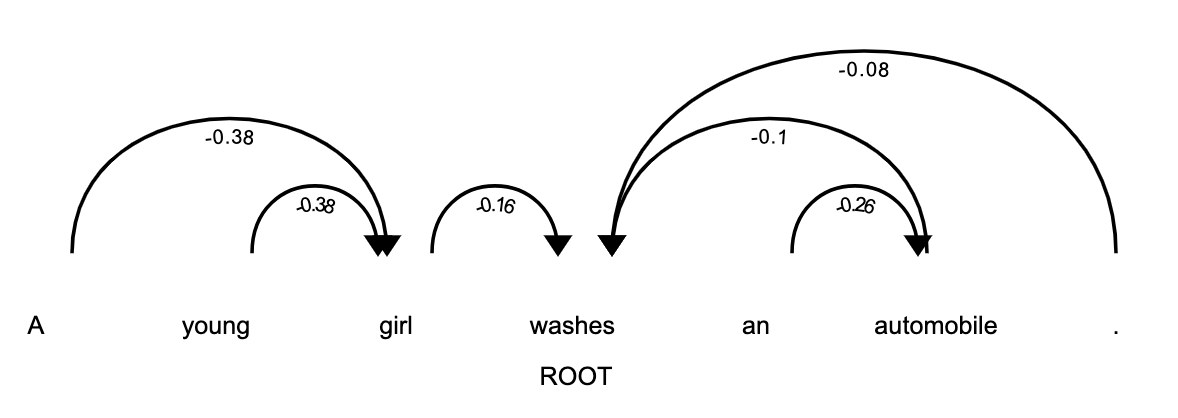
\includegraphics[width=\columnwidth]{images/all_freeze_9533.png}
        \caption{Parse obtained using the the PTB-All ($\times$) configuration.}
        \label{subfig:expl1-1}
    \end{subfigure}
    \hfill
    \begin{subfigure}[b]{0.475\textwidth}  
        \centering 
        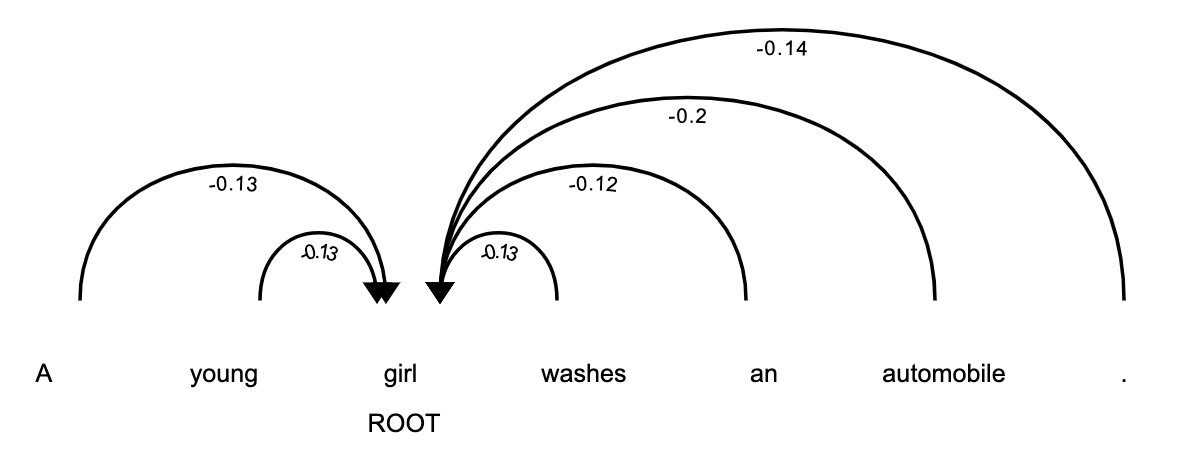
\includegraphics[width=\columnwidth]{images/all_update_9533.png}
        \caption{Parse obtained using the the PTB-All ($\checkmark$) configuration.}
        \label{subfig:expl1-2}
    \end{subfigure}
    \vskip\baselineskip
    \begin{subfigure}[b]{0.475\textwidth}   
        \centering 
        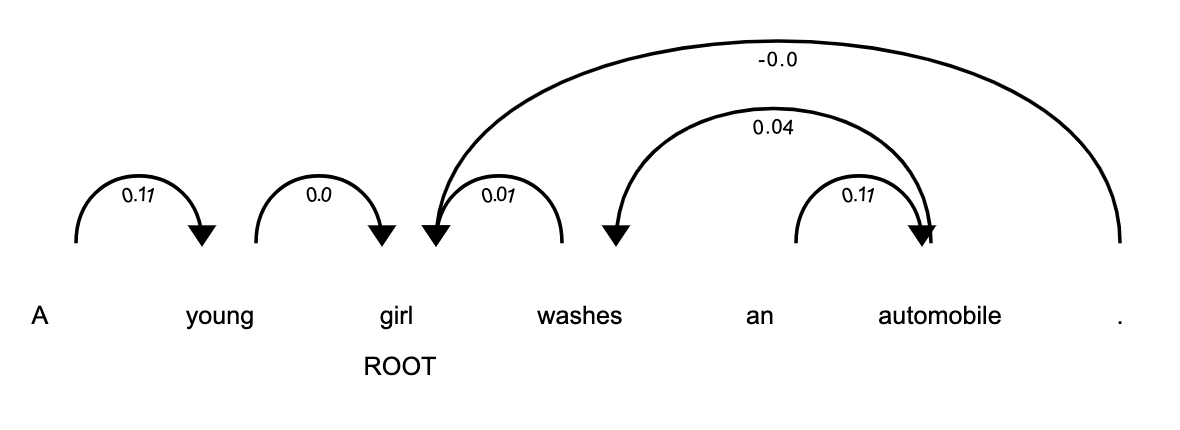
\includegraphics[width=\columnwidth]{images/100_freeze_9533.png}
        \caption{Parse obtained using the the PTB-100 ($\times$) configuration.}
        \label{subfig:expl1-3}
    \end{subfigure}
    \hfill
    \begin{subfigure}[b]{0.475\textwidth}
        \centering 
        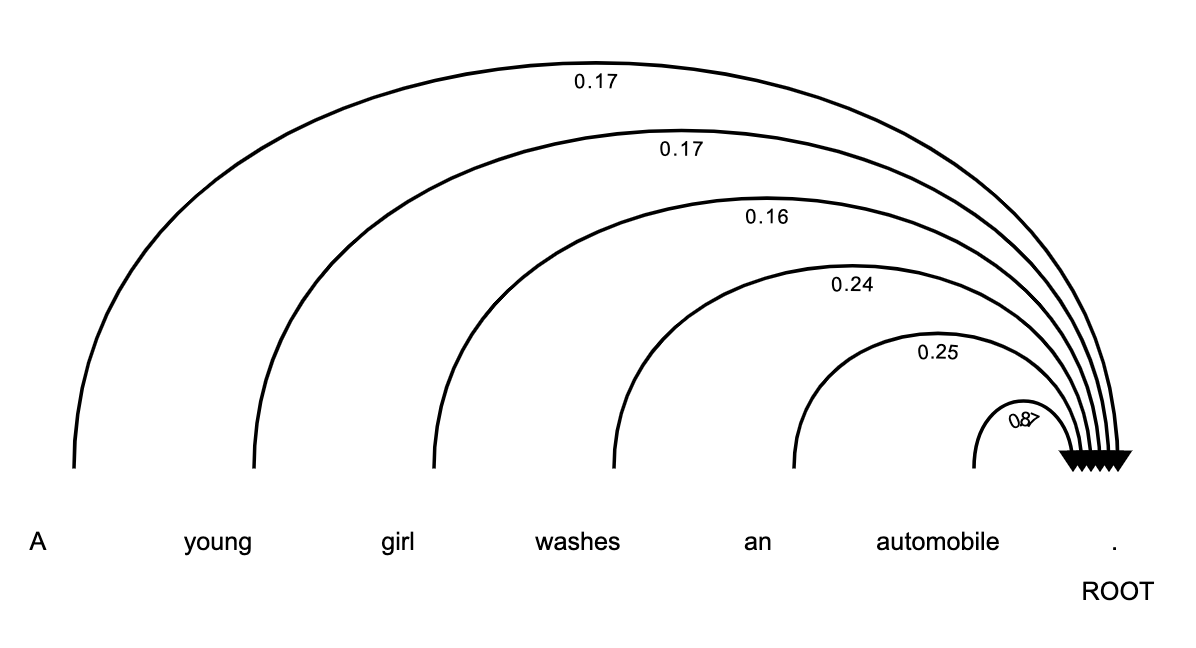
\includegraphics[width=\columnwidth]{images/100_update_9533.png}
        \caption{Parse obtained using the the PTB-100 ($\checkmark$) configuration.}
        \label{subfig:expl1-4}
    \end{subfigure}
    \vskip\baselineskip
    \begin{subfigure}[b]{0.475\textwidth}
        \centering
        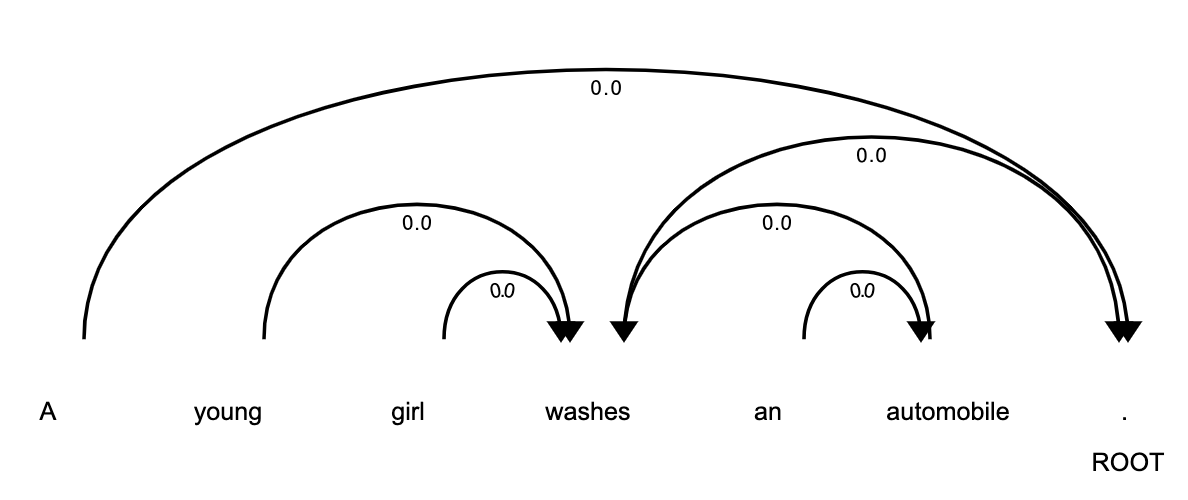
\includegraphics[width=\columnwidth]{images/bert_att_0_9533.png}
        \caption{Parse obtained using the attention head \#$1$ and without updating \textsc{Bert}.}
        \label{subfig:expl1-5}
    \end{subfigure}
    \hfill
    \begin{subfigure}[b]{0.475\textwidth}  
        \centering 
        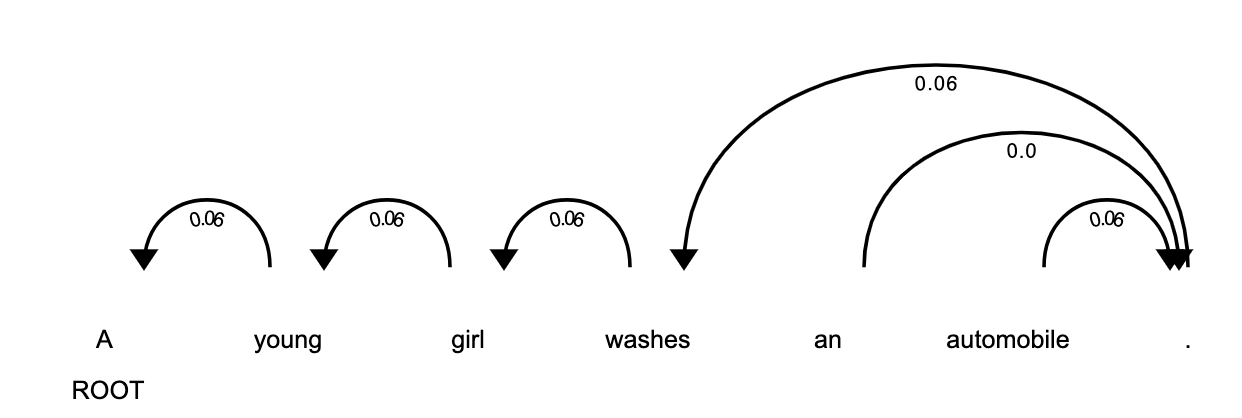
\includegraphics[width=\columnwidth]{images/bert_att_0_9533_update.png}
        \caption{Parse obtained using the attention head \#$1$ and updating \textsc{Bert}.}
        \label{subfig:expl1-6}
    \end{subfigure}
    \caption{Example of parse obtained using various configurations from our model. The parser component is initialized on PTB-All (\ref{subfig:expl1-1}, \ref{subfig:expl1-2}), PTB-100 (\ref{subfig:expl1-3}, \ref{subfig:expl1-4}) or \textsc{Bert} (\ref{subfig:expl1-5}, \ref{subfig:expl1-6}). We either freeze ($\times$) or update ($\checkmark$) the parser during the fine tuning on the SNLI. We include the weights $\alpha$ produced from the parser. 
    %We use \bert{} to obtain tree structures and evaluate the full pipeline on the \textbf{SICK-R} and \textbf{SNLI} tasks. 
    We report the accuracy from a single run on the test set.} 
    \label{fig:parse-expl}
\end{figure}

As a result of the fine-tuning, we observe that trees evolve into trivial structures and tend to connect every node to an arbitrary root. We postulate that such trivial structures present advantages from a computational standpoint. \textcite{shi_18} also observe that trivial trees without syntax yield better results than syntax and latent trees. They postulate that balanced binary trees benefit from two advantages. First, balanced trees treat all leaf nodes equally, making it easier to select essential information from all words within a sentence automatically. Second, balanced trees have shorter tree depths, which induces a shorter path for propagating information from leaves to roots, thereby reducing propagation errors.

For \textsc{Bert} parser initialization, we observe the fine-tuning produces rather sequential patterns, with words connected to direct neighbors. Some isolated groups of words also present inner connections.

%In our full supervised setup, we observe the parser's fine-tuning enables the model to adjust the parse from Figure~\ref{subfig:expl1-1} into the structure represented in Figure~\ref{subfig:expl1-2}. The obtained structure does match the one produced using more pre-training samples from the PTB dataset.

%In our low supervised setup, fine-tuning the parser 
%Regarding the parses obtained without any pre-training on the PTB (Figure~\ref{subfig:expl1-14), we observe all nodes tend to be connected to an arbitrarily chosen root.


%%%%%%%%%%%%%%%%%%%%%%%%%%%%%%%%%%%%%%%%%%%%%%%%%%%%%%%%%%%%%%%%%%%%%%%%%%%%%%%%%%%%%%%%
% 2. Shi
%%%%%%%%%%%%%%%%%%%%%%%%%%%%%%%%%%%%%%%%%%%%%%%%%%%%%%%%%%%%%%%%%%%%%%%%%%%%%%%%%%%%%%%%

% \textcolor{blue}{\citet{williams_18} investigate the trees produced by \citet{yogatama_17} and \citet{choi_18}. The authors show neither method produce meaningful latent trees in syntax. Moreover, Gumbel softmax outputs inconsistent latent trees across initializations while reinforcement learning outputs trivial left-branching trees. We also observe that random initialization leads to trivial trees (PTB-$\emptyset$). The PTB-100 appears as good trade off. Indeed the induced trees are close to silver references and thus meaningful regarding dependency structure. The trees are also specific to the task due to the parser fine-tuning with downstream objective.}

\subsection{Impact of the initialization on downstream tasks} % Reducing the need for annotation
\label{sec:dowstream-impact}

We observed in previous Section~\ref{sec:parses-impact} that the initialization and the training configuration of the parser component deeply impact the resulting parses. We now study the impact of the parser initialization on downstream performances.

%\paragraph{Initialization with human annotated data} % Reducing the need for annotation
% First, we consider the configurations introduced in Section~\ref{sec:parses-analysis} and study the impact of the parser initialization on downstream tasks. 

\begin{table}[!htb]
\centering
\small
\begin{tabularx}{\textwidth}{@{}Y Y | Y Y@{} }
\toprule
\textbf{PTB sample size} & \textbf{Parser fine-tuning} & \textbf{SICK-R ($r$)} & \textbf{SNLI (Acc.)} \\
\midrule
\midrule 
\multicolumn{4}{c}{\textit{Linguistic annotations}}\\
\midrule
% PTB-$\emptyset$ & $\checkmark$ & 85.6 \scriptsize{(0.6)} & 81.5 \scriptsize{(0.2)}\\
% \midrule 
% PTB-100 & $\times$  & 86.6 \scriptsize{(0.2)} & 81.9 {\scriptsize (0.3)}\\
% PTB-100 & $\checkmark$ & 86.9 \scriptsize{(0.4)} & 82.6 {\scriptsize (0.2)}\\
% \midrule
% PTB-All & $\times$  & 87.2 \scriptsize{(0.2)} & 81.9 {\scriptsize (0.6)}\\
% PTB-All & $\checkmark$ & 87.5 \scriptsize{(0.4)} & 83.0 {\scriptsize (0.2)}\\
PTB-$\emptyset$ & $\checkmark$ & 85.6 \scriptsize{(85.6)} & 84.6 \scriptsize{(85.5)}\\
\midrule 
PTB-100 & $\times$  & 86.4 \scriptsize{(86.6)} & 84.5 {\scriptsize (85.5)}\\
PTB-100 & $\checkmark$ & 86.5 \scriptsize{(86.9)} & 84.9 {\scriptsize (85.8)}\\
\midrule
PTB-All & $\times$  & 86.8 \scriptsize{(87.2)} & 85.0 {\scriptsize (85.8)}\\
PTB-All & $\checkmark$ & 87.0 \scriptsize{(87.5)} & 85.0 {\scriptsize (85.5)}\\
\midrule 
\multicolumn{4}{c}{\textit{Unsupervised parser}}\\
\midrule
% avec la taille de batch de 16
% \bert{} & $\times$  & --- & 84.4 {\scriptsize (85.3)}\\
% \bert{} & $\checkmark$ & --- & 84.1 {\scriptsize (84.5)}\\
% avec la taille de batch de 128
\textsc{Bert} & $\times$  & --- & 84.4 {\scriptsize (85.3)}\\
\textsc{Bert} & $\checkmark$ & --- & 84.6 {\scriptsize (85.1)}\\
\bottomrule
\end{tabularx}
\caption{Impact of the parser initialization on downstream task performance:  We pre-train the parser module with a given sample size from the PTB. We either freeze (\textbf{$\times$}) or update (\textbf{$\checkmark$}) the parser during the fine-tuning. We report the average score test set from 5 runs for SICK-R and 2 runs for SNLI (the score from the development set are in parentheses). We report Pearson correlation by convention as $r \times 100$.}
\label{table:parser}
\end{table}

In Table~\ref{table:parser}, we compare the impact of the different initializations for both tasks. For each setup, we report the Pearson correlation on the test set of the SICK-R task and the accuracy on the test set from the SNLI task.

We either freeze the parser component or continue to update it, given the downstream loss for each initialization. Fine-tuning the parser on the task generally leads to an improvement in the downstream results. In that regard, we share the observation from other latent tree learning methods \parencite{maillard_19, choi_18}; models jointly learning the parsing and composition function outperform those with a fixed structure. 

We also observe that models using the full or partial annotated data outperform models relying on the sole downstream supervision (PTB-$\emptyset$). This observation is more clear on the SICK-R task. We previously observed that fine-tuning the parser can lead to tree structure diverging from linguistic patterns. Nonetheless, human annotations appear to be a good initialization for our model regarding the downstream performances. 

% For technical reasons, we had to limit the batch size to 16 when fine-tuning \textsc{Bert} parsing module. Therefore, the benefit from fine-tuning the parser when using \textsc{Bert} is difficult to interpret. However, 
We can observe that models relying on linguistic-driven structures achieve better performances. Nonetheless, the difference is thin, and we present an average score across trees obtained from all attention heads. Therefore some attention heads might present structures as efficient as linguistic patterns.

\section{Conclusion and future work}

We evaluate our model on textual entailment and semantic similarity tasks. Regarding the textual similarity task, we show that our setup is competitive with \textsc{Bert} base, although the latest is trained on datasets many orders of magnitude larger. We explore to which extent the trees produced by our model compare with linguistic structures and how this initialization impacts downstream performances. We empirically observe that downstream supervision troubles producing stable parses and preserving linguistically relevant structures.  % We corroborate that the sole use of downstream supervision is insufficient to produce parses that are easy to interpret. 
To encourage convergence towards readable linguistic structures, we examine a number of initialization setups. Depending on the optimization setup, the parse tree may present instability. We also observe that our structures often converge toward trivial branching patterns, which have little in common with gold linguistic parses. However, with respect to the downstream performances, linguistic insights appear to be a relevant initialization.